%%%%%%%%%%%%%%%%%%%%%%%%%%%%%%%%%%%%%%%%%
% Wenneker Assignment
% LaTeX Template
% Version 2.0 (12/1/2019)
%
% This template originates from:
% http://www.LaTeXTemplates.com
%
% Authors:
% Vel (vel@LaTeXTemplates.com)
% Frits Wenneker
%
% License:
% CC BY-NC-SA 3.0 (http://creativecommons.org/licenses/by-nc-sa/3.0/)
% 
%%%%%%%%%%%%%%%%%%%%%%%%%%%%%%%%%%%%%%%%%

%----------------------------------------------------------------------------------------
%	PACKAGES AND OTHER DOCUMENT CONFIGURATIONS
%----------------------------------------------------------------------------------------

\documentclass[14pt]{scrartcl} % Font size

%%%%%%%%%%%%%%%%%%%%%%%%%%%%%%%%%%%%%%%%%
% Wenneker Assignment
% Structure Specification File
% Version 2.0 (12/1/2019)
%
% This template originates from:
% http://www.LaTeXTemplates.com
%
% Authors:
% Vel (vel@LaTeXTemplates.com)
% Frits Wenneker
%
% License:
% CC BY-NC-SA 3.0 (http://creativecommons.org/licenses/by-nc-sa/3.0/)
% 
%%%%%%%%%%%%%%%%%%%%%%%%%%%%%%%%%%%%%%%%%

%----------------------------------------------------------------------------------------
%	PACKAGES AND OTHER DOCUMENT CONFIGURATIONS
%----------------------------------------------------------------------------------------
\usepackage{listings}
\usepackage{color}

\definecolor{dkgreen}{rgb}{0,0.6,0}
\definecolor{gray}{rgb}{0.5,0.5,0.5}
\definecolor{mauve}{rgb}{0.58,0,0.82}

\lstset{frame=tb,
  language=Python,
  aboveskip=3mm,
  belowskip=3mm,
  showstringspaces=false,
  columns=flexible,
  basicstyle={\small\ttfamily},
  numbers=none,
  numberstyle=\tiny\color{gray},
  keywordstyle=\color{blue},
  commentstyle=\color{dkgreen},
  stringstyle=\color{mauve},
  breaklines=true,
  breakatwhitespace=true,
  tabsize=3
}

\usepackage{amsmath, amsfonts, amsthm} % Math packages

\usepackage{xcolor}

\usepackage{hyperref}

\usepackage{verbatim}

\usepackage{listings} % Code listings, with syntax highlighting

\usepackage[english]{babel} % English language hyphenation

\usepackage{graphicx} % Required for inserting images
\graphicspath{{Figures/}{./}} % Specifies where to look for included images (trailing slash required)

\usepackage{booktabs} % Required for better horizontal rules in tables

\numberwithin{equation}{section} % Number equations within sections (i.e. 1.1, 1.2, 2.1, 2.2 instead of 1, 2, 3, 4)
\numberwithin{figure}{section} % Number figures within sections (i.e. 1.1, 1.2, 2.1, 2.2 instead of 1, 2, 3, 4)
\numberwithin{table}{section} % Number tables within sections (i.e. 1.1, 1.2, 2.1, 2.2 instead of 1, 2, 3, 4)

\setlength\parindent{0pt} % Removes all indentation from paragraphs

\usepackage{enumitem} % Required for list customisation
\setlist{noitemsep} % No spacing between list items

%----------------------------------------------------------------------------------------
%	DOCUMENT MARGINS
%----------------------------------------------------------------------------------------

\usepackage{geometry} % Required for adjusting page dimensions and margins

\geometry{
	paper=a4paper, % Paper size, change to letterpaper for US letter size
	top=2.5cm, % Top margin
	bottom=3cm, % Bottom margin
	left=3cm, % Left margin
	right=3cm, % Right margin
	headheight=0.75cm, % Header height
	footskip=1.5cm, % Space from the bottom margin to the baseline of the footer
	headsep=0.75cm, % Space from the top margin to the baseline of the header
	%showframe, % Uncomment to show how the type block is set on the page
}

%----------------------------------------------------------------------------------------
%	FONTS
%----------------------------------------------------------------------------------------

\usepackage[utf8]{inputenc} % Required for inputting international characters
\usepackage[T1]{fontenc} % Use 8-bit encoding

\usepackage{fourier} % Use the Adobe Utopia font for the document

%----------------------------------------------------------------------------------------
%	SECTION TITLES
%----------------------------------------------------------------------------------------

\usepackage{sectsty} % Allows customising section commands

\sectionfont{\vspace{6pt}\centering\normalfont\scshape} % \section{} styling
\subsectionfont{\normalfont\bfseries} % \subsection{} styling
\subsubsectionfont{\normalfont\itshape} % \subsubsection{} styling
\paragraphfont{\normalfont\scshape} % \paragraph{} styling

%----------------------------------------------------------------------------------------
%	HEADERS AND FOOTERS
%----------------------------------------------------------------------------------------

\usepackage{scrlayer-scrpage} % Required for customising headers and footers

\ohead*{} % Right header
\ihead*{} % Left header
\chead*{} % Centre header

\ofoot*{} % Right footer
\ifoot*{} % Left footer
\cfoot*{\pagemark} % Centre footer
 % Include the file specifying the document structure and custom commands

%----------------------------------------------------------------------------------------
%	TITLE SECTION
%----------------------------------------------------------------------------------------



\title{	
	\normalfont\normalsize
	\textsc{Programação de Sistemas Embarcados}\\ % Your university, school and/or department name(s)
	\vspace{25pt} % Whitespace
	\rule{\linewidth}{0.5pt}\\ % Thin top horizontal rule
	\vspace{20pt} % Whitespace
	{\huge Visão de Máquina aplicada a contagem de carros}\\ % The assignment title
	\vspace{12pt} % Whitespace
	\rule{\linewidth}{2pt}\\ % Thick bottom horizontal rule
	\vspace{12pt} % Whitespace
}

\author{\LARGE Rodrigo Bandeira} % Your name

\date{\normalsize\today} % Today's date (\today) or a custom date

\begin{document}

\maketitle % Print the title

%----------------------------------------------------------------------------------------
%	FIGURE EXAMPLE
%----------------------------------------------------------------------------------------

\begin{figure}[h] % [h] forces the figure to be output where it is defined in the code (it suppresses floating)
	\centering
	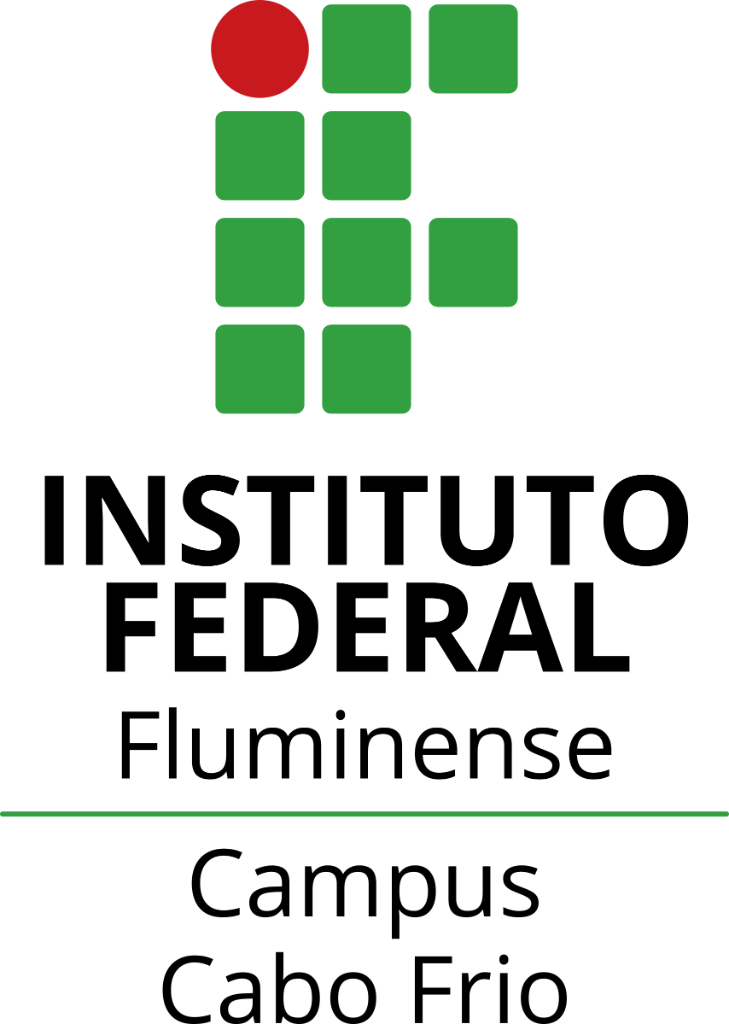
\includegraphics[width=0.5\columnwidth]{iff.png} % Example image
\end{figure}

\newpage

\section{Resumo}
	O projeto consiste na contagem de carros que passam em uma rua qualquer. O algoritmo tem a intenção de ser em tempo real. É planejado que o computador com uma camera tenha contato Wireless com um aparelho celular de sistema operacional Android. 

\section{Objetivos}
	O objetivo do projeto é de permitir a automatização da contagem de carros que passam por uma rua qualquer, a partir de uma camera conectada a um mini-computador, estou planejando usar o Raspberry Pi, por ter o poder computacional um pouco maior que o Arduíno. A interface do aplicativo deve contar com a camera, em tempo real ou não, e um contador de veículos. A princípio, estou planejando apenas contar quantos carros passam pela rua, mas caso for possível, também será contado a quantidade de outros tipos de veículos estão passando pela rua.
\newline 	Estou pensando em usar um algoritmo de machine learning, o que ocasionaria na chance de uma imagem captada ser um veículo. Logo, teria uma margem de erro para a detecção de carros. Espero que essa margem de erro seja de no máximo 1\%. \newline
	A base de todo o algoritmo a ser utilizado vai ser a correlação de imagens, que é basicamente a extrapolação da correlação, mas agora em uma matriz bi-dimensional.  A correlação bi-dimensional $r_{ij}$ pode ser descrita da seguinte maneira:  \newline
\begin{equation}
\label{eq:primitiva}
r_{ij}=\frac{\sum_{m}\sum_{n}[f(m+i,n+j)-\bar{f}][g(m,n)-\bar{g}]}{\sqrt{\sum_{m}\sum_{n}f(m,n)-\bar{f}]^{2}\sum_{m}\sum_{n}[g(m,n)-\bar{g}]^2}}
\end{equation}
	O gráfico 3D de quantidade de correlação pode ser obtido a partir da seguinte matriz:
\begin{equation}
\label{eq:def}
x* = x+u+\frac{\partial u}{\partial x} \Delta x+\frac{\partial u}{\partial y}\Delta y
\end{equation}
\newline
\begin{equation}
\label{eq:def}
y* = y+v+\frac{\partial v}{\partial x} \Delta x+\frac{\partial v}{\partial y}\Delta y
\end{equation}
\section{Justificativa}
\subsection{Geral}
	A maior motivação para este projeto foi o fato de ter tido um estágio no Instituto, na qual os estagiandos tinham que manualmente contar quantos carros estavam passando pela rua, o que é extremamente gastante, e existe uma grande possibilidade de erro humano, já que ao anotar vários tipos de veículos diferentes durante o período de 8 horas, os humanos ficam cansados e acabam fazendo o trabalho de qualquer jeito, causando grande imprecisão nos dados coletados. \newline
	Outro objetivo do trabalo é aperfeicoar a habilidade do aluno com sistemas embarcados e algoritmos de visão computacional, a fim de ser um engenheiro mecânico mais capacitado e melhor adaptado a indústria moderna que estamos vivendo.

\subsection{Específicos}
Os materiais físicos que pretendo usar para esse projeto são:
\begin{itemize}
  \item Raspberry Pi
  \item Módulo de Camera para Raspberry
  \item Cartão de memória de capacidade para gravar algumas horas.
\end{itemize}

Os softwares que pretendo usar para esse projeto são:
\begin{itemize}
  \item OpenCV com C++
  \item OpenCV com Python
  \item Visual Studio Code
  \item Raspbian
\end{itemize}

\newpage
\section{Fluxograma}
\begin{figure}[h]
	\centering
	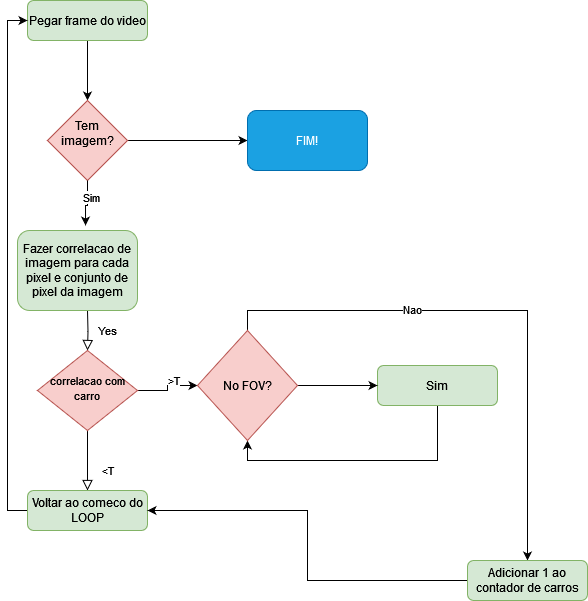
\includegraphics[width=1\columnwidth]{fluxograma.png}
\end{figure}

\end{document}
